% Template for PLoS
% Version 3.1 February 2015
%
% To compile to pdf, run:
% latex plos.template
% bibtex plos.template
% latex plos.template
% latex plos.template
% dvipdf plos.template
%
% % % % % % % % % % % % % % % % % % % % % %
%
% -- IMPORTANT NOTE
%
% This template contains comments intended 
% to minimize problems and delays during our production 
% process. Please follow the template instructions
% whenever possible.
%
% % % % % % % % % % % % % % % % % % % % % % % 
%
% Once your paper is accepted for publication, 
% PLEASE REMOVE ALL TRACKED CHANGES in this file and leave only
% the final text of your manuscript.
%
% There are no restrictions on package use within the LaTeX files except that 
% no packages listed in the template may be deleted.
%
% Please do not include colors or graphics in the text.
%
% Please do not create a heading level below \subsection. For 3rd level headings, use \paragraph{}.
%
% % % % % % % % % % % % % % % % % % % % % % %
%
% -- FIGURES AND TABLES
%
% Please include tables/figure captions directly after the paragraph where they are first cited in the text.
%
% DO NOT INCLUDE GRAPHICS IN YOUR MANUSCRIPT
% - Figures should be uploaded separately from your manuscript file. 
% - Figures generated using LaTeX should be extracted and removed from the PDF before submission. 
% - Figures containing multiple panels/subfigures must be combined into one image file before submission.
% For figure citations, please use "Fig." instead of "Figure".
% See http://www.plosone.org/static/figureGuidelines for PLOS figure guidelines.
%
% Tables should be cell-based and may not contain:
% - tabs/spacing/line breaks within cells to alter layout or alignment
% - vertically-merged cells (no tabular environments within tabular environments, do not use \multirow)
% - colors, shading, or graphic objects
% See http://www.plosone.org/static/figureGuidelines#tables for table guidelines.
%
% For tables that exceed the width of the text column, use the adjustwidth environment as illustrated in the example table in text below.
%
% % % % % % % % % % % % % % % % % % % % % % % %
%
% -- EQUATIONS, MATH SYMBOLS, SUBSCRIPTS, AND SUPERSCRIPTS
%
% IMPORTANT
% Below are a few tips to help format your equations and other special characters according to our specifications. For more tips to help reduce the possibility of formatting errors during conversion, please see our LaTeX guidelines at http://www.plosone.org/static/latexGuidelines
%
% Please be sure to include all portions of an equation in the math environment.
%
% Do not include text that is not math in the math environment. For example, CO2 will be CO\textsubscript{2}.
%
% Please add line breaks to long display equations when possible in order to fit size of the column. 
%
% For inline equations, please do not include punctuation (commas, etc) within the math environment unless this is part of the equation.
%
% % % % % % % % % % % % % % % % % % % % % % % % 
%
% Please contact latex@plos.org with any questions.
%
% % % % % % % % % % % % % % % % % % % % % % % %

\documentclass[10pt,letterpaper]{article}
\usepackage[top=0.85in,left=2.75in,footskip=0.75in]{geometry}

% Use adjustwidth environment to exceed column width (see example table in text)
\usepackage{changepage}

% Use Unicode characters when possible
\usepackage[utf8]{inputenc}

% textcomp package and marvosym package for additional characters
\usepackage{textcomp,marvosym}

% fixltx2e package for \textsubscript
\usepackage{fixltx2e}

% amsmath and amssymb packages, useful for mathematical formulas and symbols
\usepackage{amsmath,amssymb}

% cite package, to clean up citations in the main text. Do not remove.
\usepackage{cite}

% Use nameref to cite supporting information files (see Supporting Information section for more info)
\usepackage{nameref,hyperref}

% line numbers
\usepackage[right]{lineno}

% ligatures disabled
\usepackage{microtype}
%\DisableLigatures[f]{encoding = *, family = * }

% rotating package for sideways tables
\usepackage{rotating}

\usepackage{tikz}
\usepackage{subfig}
\usepackage{algorithm}
\usepackage{algpseudocode}
\usepackage{calc}
\usepackage{siunitx}
%\usepackage{graphics}


% Remove comment for double spacing
%\usepackage{setspace} 
%\doublespacing

% Text layout
\raggedright
\setlength{\parindent}{0.5cm}
\textwidth 5.25in 
\textheight 8.75in

% Bold the 'Figure #' in the caption and separate it from the title/caption with a period
% Captions will be left justified
\usepackage[aboveskip=1pt,labelfont=bf,labelsep=period,justification=raggedright,singlelinecheck=off]{caption}

% Use the PLoS provided BiBTeX style
\bibliographystyle{plos2015}

% Remove brackets from numbering in List of References
\makeatletter
\renewcommand{\@biblabel}[1]{\quad#1.}
\makeatother

% Leave date blank
\date{}

% Header and Footer with logo
\usepackage{lastpage,fancyhdr,graphicx}
\usepackage{epstopdf}
\pagestyle{myheadings}
\pagestyle{fancy}
\fancyhf{}
\lhead{\includegraphics[width=2.0in]{PLOS-submission.eps}}
\rfoot{\thepage/\pageref{LastPage}}
\renewcommand{\footrule}{\hrule height 2pt \vspace{2mm}}
\fancyheadoffset[L]{2.25in}
\fancyfootoffset[L]{2.25in}
\lfoot{\sf PLOS}

%% Include all macros below

\newcommand{\lorem}{{\bf LOREM}}
\newcommand{\ipsum}{{\bf IPSUM}}

% Generelt
\newcommand{\ud}{\mathrm{d}} % d
\newcommand{\R}{\mathbb{R}} % Real numbers
\newcommand{\T}{\mathscr{T}}

% Operatorer og funktionaler
\newcommand{\I}{\mathbb{I}} % I

\newcommand{\CE}[2]{\mathrm{E}\left[\,#1\,|\,#2\,\right]} % Conditional expectation

\newcommand{\by}{\boldsymbol{y}}
\newcommand{\bc}{\boldsymbol{c}}
\newcommand{\bd}{\boldsymbol{d}}
\newcommand{\bP}{\boldsymbol{\Phi}}
\newcommand{\bZ}{Z}%{\boldsymbol{Z}}
\newcommand{\bV}{V}%{\boldsymbol{V}}
\newcommand{\br}{\boldsymbol{r}}
\newcommand{\bt}{\boldsymbol{t}}
\newcommand{\btheta}{\boldsymbol{\vartheta}}
\newcommand{\bht}{\hat{\boldsymbol{\vartheta}}}
\newcommand{\bz}{\boldsymbol{z}}
\newcommand{\bx}{{\boldsymbol{x}}}
\newcommand{\bv}{v}
\newcommand{\bw}{\boldsymbol{w}}
\newcommand{\vv}{\boldsymbol{v}}
\newcommand{\bepsilon}{\boldsymbol{\varepsilon}}

%% END MACROS SECTION

\setcounter{secnumdepth}{3}
\begin{document}
\vspace*{0.35in}

% Title must be 250 characters or less.
% Please capitalize all terms in the title except conjunctions, prepositions, and articles.
\begin{flushleft}
{\Large
\textbf\newline{Neuron's Eye View: Inferring Features of Complex Stimuli from Neural Responses} % Please use "title case" (capitalize all terms in the title except conjunctions, prepositions, and articles).
}
\newline
% Insert author names, affiliations and corresponding author email (do not include titles, positions, or degrees).
\\
Xin (Cindy) Chen\textsuperscript{1},
Jeffrey M. Beck\textsuperscript{2},
John M. Pearson\textsuperscript{1*},
\\
\bigskip
\textbf{1} Duke Institute for Brain Sciences, Duke University, Durham, North Carolina, USA
\\
\textbf{2} Department of Neurobiology, Duke University Medical Center, Durham, North Carolina, USA
\\
\bigskip

% Insert additional author notes using the symbols described below. Insert symbol callouts after author names as necessary.
% 
% Remove or comment out the author notes below if they aren't used.
%
% Primary Equal Contribution Note
%\Yinyang These authors contributed equally to this work.

% Deceased author note
%\dag Deceased

% Group/Consortium Author Note
%\textpilcrow Membership list can be found in the Acknowledgments section.

% Use the asterisk to denote corresponding authorship and provide email address in note below.
* john.pearson@duke.edu

\end{flushleft}
% Please keep the abstract below 300 words

\section*{Supporting Information}

\subsection*{Latent state model}
We model each of the latent states $z_{tk}$ as an independent Markov process for each feature $k$. That is, each $k$ indexes an independent Markov chain with initial state probability $\pi_k\sim \text{Dir}(\alpha_\pi)$ and transition matrix $A_k\sim \text{Dir}(\alpha_A)$. For the semi-Markov case, we assume that the dwell times in each state are distributed independently for each chain according to an integer-valued, truncated lognormal distribution with support on the integers $1\dots D$:
\begin{align}
    \label{semi-markov}
    p_k(d|z = j) &= \text{Log-Normal}(d|m_{jk}, s^2_{jk}) / W_{jk}  \\
    W_{jk} &= \sum_{d = 1}^D \text{Log-Normal}(d|m_{jk}, s^2_{jk}) 
\end{align}
Note that we have allowed the dwell time distribution to depend on both the feature $k$ and the state of the Markov chain $j$. In addition, we put indpendent Normal-Gamma priors on the mean $(m_{kj})$ and precision $(\tau_{kj} \equiv s_{kj}^{-2})$ parameters of the distribution: $(m, \tau) \sim \text{NG}(\mu, \lambda, \alpha, \beta)$.

\subsection*{Autocorrelated noise in natural time}
In order to model the potential correlation of firing rates in consecutive times, we included the moment-by-moment fluctuation in the firing rate of each unit:
\begin{equation}
    (\lambda_{\mathrm{eff}})_{tu} = \prod_k \theta_{\tau u} \lambda_{ku}^{z_{tk}}
\end{equation}
where $\tau$ is the natural time when a movie clip is played.

Further, we assume the overdispersion parameter $\theta_{\tau u} = \phi_{\tau u} \theta_{\tau - 1, u}$ is modulated by $\phi$ from the last moment. Let $\phi_{0u} = \theta_{0, u}$, then we have $\theta_{\tau u} = \prod_{\tau' \le \tau} \phi_{\tau' u}$.



\subsection*{Movie data}
Finally, we applied our model to a data set comprising single neuron recordings made in macaque monkeys as they freely viewed movies of primate social interactions in the wild%\cite{adams_inprep}
 . These video clips, collected from a rhesus macaque research field site, effectively represent the range of behaviorally relevant stimuli for macaques, including the four ``F''s of animal behavior: fighting, fleeing, foraging, and reproduction. Thus this dataset represents a rare opportunity for exploratory feature selection based on neural responses.

On each trial of the experiment, monkeys viewed a random 5-second clip from a movie database ($T \approx 5$h, $dt = 30$ frames/s). On the following trial, monkeys were given a two-alternative choices with options chosen from the set \{repeat clip, continue clip, blank screen, new clip\}. Since each neuron saw only a subset of clips within the database, and these clips began at with random offsets, observations were sparse, with total number of observations $N_{obs} = 7.42 \times 10^6$ and $\overline{M} = N_{obs}/T \approx 14$. These data form a particularly intriguing application of our model, since the neurons recorded were located in the orbitofrontal and dorsolateral prefrontal cortices, areas not normally associated with low-level visual processing. In fact, there is reason to believe that the relevant features encoded in these areas for such naturalistic stimuli are behavioral and social \cite{watson2012social}.

Because the behaviors of interest in these stimuli potentially span a large range of time scales, we used semi-Markov dynamics with a maximum duration of $D = 500$ on the latent states\footnote{We also allowed for self-transitions, potentially capturing behavior on even longer timescales.}. We fit a model with $K=10$ features and the same hierarchical priors on baselines and latent firing rate effects as in previous experiments. In addition, because many neurons in the data set exhibited a transitory increase in firing with movie onset on each trial (independent of movie content), we include this movie onset response as an external covariate $x(t)$ specific to each neuron. We calculated this separately for each recorded unit by averaging spike counts (relative to stimulus onset) across trials, smoothing, and taking the log so that $x(t)$ was coded as a multiplicative rather than an additive effect on firing. This can be loosely viewed as a means of preprocessing our data, in which we account for a large known effect by specifying it as a covariate in the model.

% Place figure captions after the first paragraph in which they are cited.
\begin{figure}[!h]
    \center
    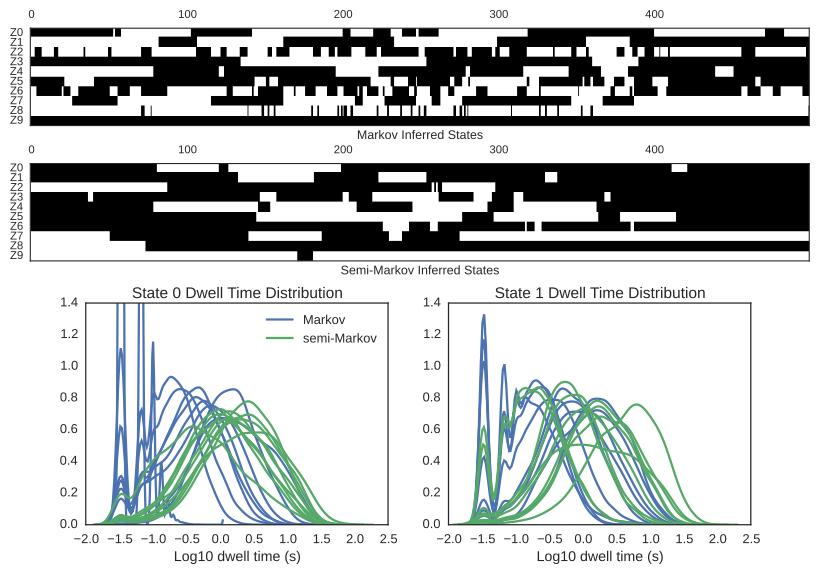
\includegraphics[width=\linewidth]{figures/movie_data}
	\caption{\bf Inferred states of the movie dataset.}
	A: Maximum \emph{a posterior} inferred features for the Markov and semi-Markov models. Plotted data are for the same stimulus for $\approx 17$s of data. B: Estimated dwell time distributions for off (0) and on (1) states in the Markov and semi-Markov models. Dwell times include self-transitions. Dwell times for the Markov case (blue) are clearly lower than those for the semi-Markov case (green).
	\label{movie_results}
\end{figure}

Figure \ref{movie_results} shows a comparison of Markov and semi-Markov models applied to feature detection in the stimulus set. Labels were calculated as maxima of posterior marginals, independently for each time bin. Clearly, the semi-Markov model captures the rich heterogeneity in the durations of stimulus-driven features in neural spiking, particularly in the on (1) state. This is also visible in the kernel density estimates, which show event durations on the order of tens of seconds for the semi-Markov model, as opposed to mere seconds in the Markov case. Thus semi-Markov models (and other models that take into account multiple timescales) will likely be necessary to capture variations in neural activity on the timescales relevant to natural behaviors.




\nolinenumbers

%\section*{References}
% Either type in your references using
% \begin{thebibliography}{}
% \bibitem{}
% Text
% \end{thebibliography}
%
% OR
%
% Compile your BiBTeX database using our plos2015.bst
% style file and paste the contents of your .bbl file
% here.
% 
%\bibliography{bib.bib}
\begin{thebibliography}{10}

\bibitem{watson2012social}
K. K. Watson and M. L. Platt.
\newblock Social signals in primate orbitofrontal cortex.
\newblock Current Biology. vol. 22, no. 23, pp. 2268--2273, 2012.

\end{thebibliography}


\end{document}

